%% LyX 2.0.3 created this file.  For more info, see http://www.lyx.org/.
%% Do not edit unless you really know what you are doing.
\documentclass[12pt,english]{article}
\usepackage[latin9]{inputenc}
%\setlength{\headheight}{15pt}
%\usepackage{fancyhdr}
%\pagestyle{p}
\setcounter{secnumdepth}{3}
\setcounter{tocdepth}{3}
\usepackage{mathtools}
\usepackage{amssymb}
\usepackage{graphicx}
\usepackage{setspace}
\onehalfspacing
\usepackage[unicode=false,pdfusetitle,
 bookmarks=true,bookmarksnumbered=true,bookmarksopen=false,
 breaklinks=false,pdfborder={0 0 0},backref=false,colorlinks=false]
 {hyperref}

\makeatletter
%%%%%%%%%%%%%%%%%%%%%%%%%%%%%% User specified LaTeX commands.
\usepackage[english]{babel}
\newcommand{\BigO}[1]{\ensuremath{\operatorname{O}\bigl(#1\bigr)}}


\makeatother

\begin{document}

\title{Implemention of Reverse Time Migration on FPGA}
\author{Conghui He}

\maketitle

\tableofcontents
%include the introduction

\section{Introduction}

The goal of exploration seismology is to find oil and gas reservoirs
by seismically imaging the earth's reflectivity distribution. Towards
this goal, exploration geophysicists perform seismic experiments ideally
equivalent to that shown in Figure (\ref{fig:oil-drilling}).

\begin{figure}[h]
\centering
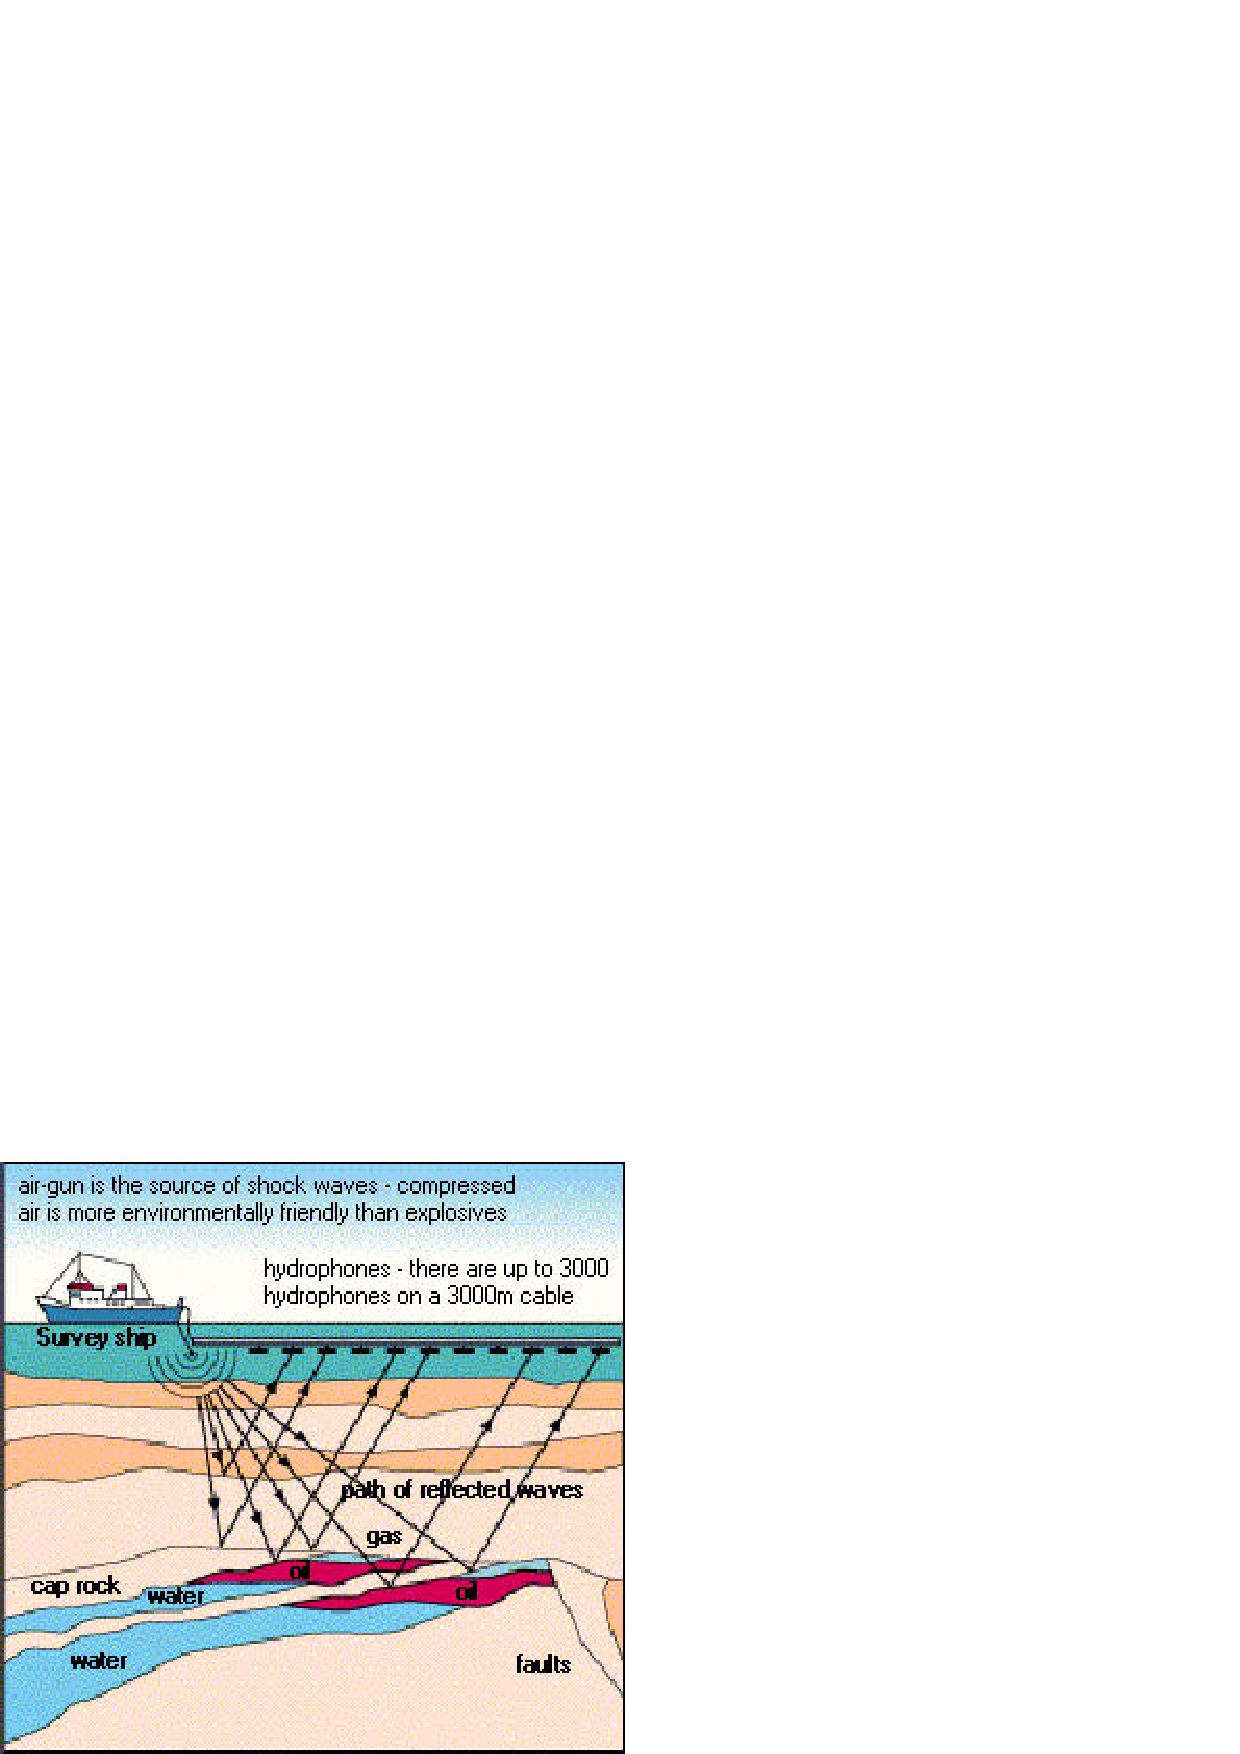
\includegraphics[scale=0.65]{img/oil-drilling-prospecting2.jpg}
\caption{Searching for oil over water using seismology}
\label{fig:oil-drilling}
\end{figure}

Here,
the survey ship excites seismic waves by its air gun, and the resulting
primary reflections are recorded by a set of hydrophones. The geologists
are the ones responsible for finding the oil trap or gas trap by processing
and analyzing the 3D wave fields that are reflected back by the subsurface.
However, only with the help of computers and engineers could the data
be processed and analyzed because terabytes of data would be processed.
The computational performance plays an important role through out
the process because the Reverse Time Migration (RTM) algorithm is
a high computational-demanding imaging algorithm.%
\footnote{The complexity of RTM for a single shot is roughly \BigO{n4}%
}



The ultimate and perhaps unattainable goal of computer science is
to make the computer to do whatever we want in perfect accuracy, speed,
security and on and on. Over time, the number of transistor on integrated
circuit doubles approximately every two year, which greatly improves
the computational performance and memory capacity of the general purpose
computer. However, as CPU speeds and memory capabilities have increased,
other aspects of performance, such as the access speed of register
and memory, or the access speed of memory and disk, have failed to
keep up. As a result, the performance of the whole system isn't likely
to improve a lot, and the access latencies frequently become a bottleneck
in the system.

Lots of efforts have been made facing with the access latencies, and
some of the methods gained extraordinary achievement. For example,
the vendors who manufacturing the chips try to use \emph {out-of-order
execution}  paradigm to make use of instruction cycles that would
be otherwise be wasted by a certain type of costly delay. One more
well-known ways to reduce the latencies between the fast-speed CPU
registers and relative-low-speed main memory is use \emph {caching.}
By storing the copy of data that are frequently accessed by the
processor into the cache, the amount of time that processors read
and write directly from/to memory decrease significantly, thus improves
the overall performance.

Such kinds of techniques, out-of-order execution, on-chip cache and
prefetching that we didn't mention before, does reduce the memory
latencies bottleneck, however, it also requires more transistors for
designing the processors, and the design of processors becomes more
and more complicated. What's worse, when the consecutive read/write
instructions cover a wide range of memory location, or the memory
access pattern is too random to predict, the application will suffer
from a high ratio of cache misses and the memory bottleneck re-emerge\cite{fu11}.

The current trend of improving the computer performance can be divided
into three category, increase the clock rate, fitting more and more
cores into a single processor, multiple computers (nodes) cooperate
together, and use some co-processors.

For years, processor makers consistently delivered increases in clock
rates and instruction-level parallelism, so that single-threaded code
executed faster on newer processors with no modification\cite{herb11}.
However, For a given device, operating at a higher clock rate always
requires more power. Especially, the high clock rate cannot be tolerated
in cluster computing or grid computing, or super computing, because
there are hundreds of thousands of processors within a cluster. That
is why the clock rate of servers servers generally stays between 2.0Ghz
and 2.4Ghz.

Now, to manage the CPU power dissipation, processor makers favor multi-core
designs, that is, integrate more than one core into a single processor,
such as the Intel Ferry CPUs, which have up to 32 cores. Following
the change of the CPU architecture, the software has also to be changed
at the same time. The previously single-thread (single-process) programs
have to be modified to multi-thread (multi-process) manner to take
full advantage of the hardware. Most of the multi-threaded development
paradigms introduce new overhead, and you will not see a linear increase
in speed vs number of processors. This is particularly true while
accessing shared or dependent resources, due to lock contention. This
effect becomes more noticeable as the number of processors increases\cite{moore}.

The computational performance for a single computer (node) is not
enough to support most of the science computation. Generally, scientists
and some of the industries would set up a \emph{cluster}, which consists
of a set of loosely connected or tightly connected computers that
work together so that in many respects they can be viewed as a single
system. Compared with a personal computer, the whole cluster certainly
has higher performance, but it also costs more power and the average
performance of a single node of the cluster is much lower than that
works individually. The entire performance of the cluster may even
increase slower when the number of nodes increase. What's more, for
a cluster, more aspects should be taken into consideration for tunning
the performance, including networking bandwidth and latency, parallel
file system performance, the application scalability and so on.

The most powerful supercomputer \emph{Titan}, which is made by Cray
Inc, has 560640 cores, 710144GB memory and it reaches high a Linpack
Performance of 17590.0 TFlops\footnote {Flops: number of double-precision
floating point operation per second} with its power being 8209kw\cite{top500}.
The scientist yet seems not content with the current computational
power because even by using the super computer, it still takes several
months or even several years to run some of simulation, such as seismic
imaging, weather simulation, ocean simulation, or global simulation.
And they need higher computational performance for a higher resolution
of the simulation.

Some vendors manufacture co-processor to aid CPU to better perform
general computing. For example, the NVIDIA Cooperation publish its
GPU accelerating card, which consists of hundreds of core in a single
card \footnote{There are 512 cores in NVIDIA Fermi GPUs}. GPU is better at general arithmetic
computation than general purpose CPU not only because it has more
cores than CPU, but also because its ratio of FLOPS  to power is much
higher than CPU. It can save lots of power in a cluster. The NVIDIA Inc
provides a set of
API, eg. CUDA C, for programmer to develop applications running on
NVIDIA card. The programs running on GPU cards are similar to the
programs running to CPU. In a word, they are both software.

Some vendors and researches still trying to increase the computational
performance as well as the ratio of FLOPS to power. You may wonder
whether we can build our application in hardware level instead of
software level, which could satisfy the vendors and researchers' willing.
That is why FPGA emerged.

A \emph {field-programmable gate array} (FPGA) is an integrated
circuit that is designed to be configured by the customer or a designer
after manufacturing, thereby \emph {field-programmable.}

The magic of FPGAs is that the connections among the logic gates (the
actual circuit you need) are made at power-up by reading the configuration
instructions written into a bit file. Changing the file changes the
function of the FPGA.

In this paper, I present my FPGA-based solution for the Reverse Time
Migration (RTM) algorithm ~\cite{yoon03}, which is the most computationally-demanding
imaging algorithms in oil and gas exploration.

The Reverse Time Migration (RTM) is a wave equation depth migration
method. It offers insights into geology that were previously impossible
to interpret or understand using seismic data.

Conventional migration methods, generally, use standard wave equation
techniques with mathematical approximations assuming that wave field
propagate in only one field. RTM is a two-way migration solution that
more accurately implements the wave equation and provides an alternative
approach to migration with fewer compromises. RTM works by running
the wave equation forward in time for the source and backwards in
time for the receiver ~\cite{shafiq}.

The RTM algorithm generally needs to deal with source and receiver
3D wave field arrays at thousands of different time steps, which brings
the requirement to manipulate terabytes of data in disk or in memory.
The kernel of the RTM algorithm, which applies a large 3D stencil
over a 3D data cube, needs to access a wide range of memory locations
while computing the result of one point. In many cases, the computation
incurs a large number of cache misses and reduces the performance
significantly. These highly demanding memory access characteristics
of RTM form a 'memory wall' that keeps us from achieving high throughput
in common computer clusters ~\cite{fu11}.

In this work, by utilizing the great computing performance of FPGA
and enormous internal memory bandwidth of the FPGA, I manage to implement
the computationally-demanding Reverse Time Migration algorithm in
FPGA.

%
\section{Introduction}

The goal of exploration seismology is to find oil and gas reservoirs
by seismically imaging the earth's reflectivity distribution. Towards
this goal, exploration geophysicists perform seismic experiments ideally
equivalent to that shown in Figure (\ref{fig:oil-drilling}).

\begin{figure}[h]
\centering
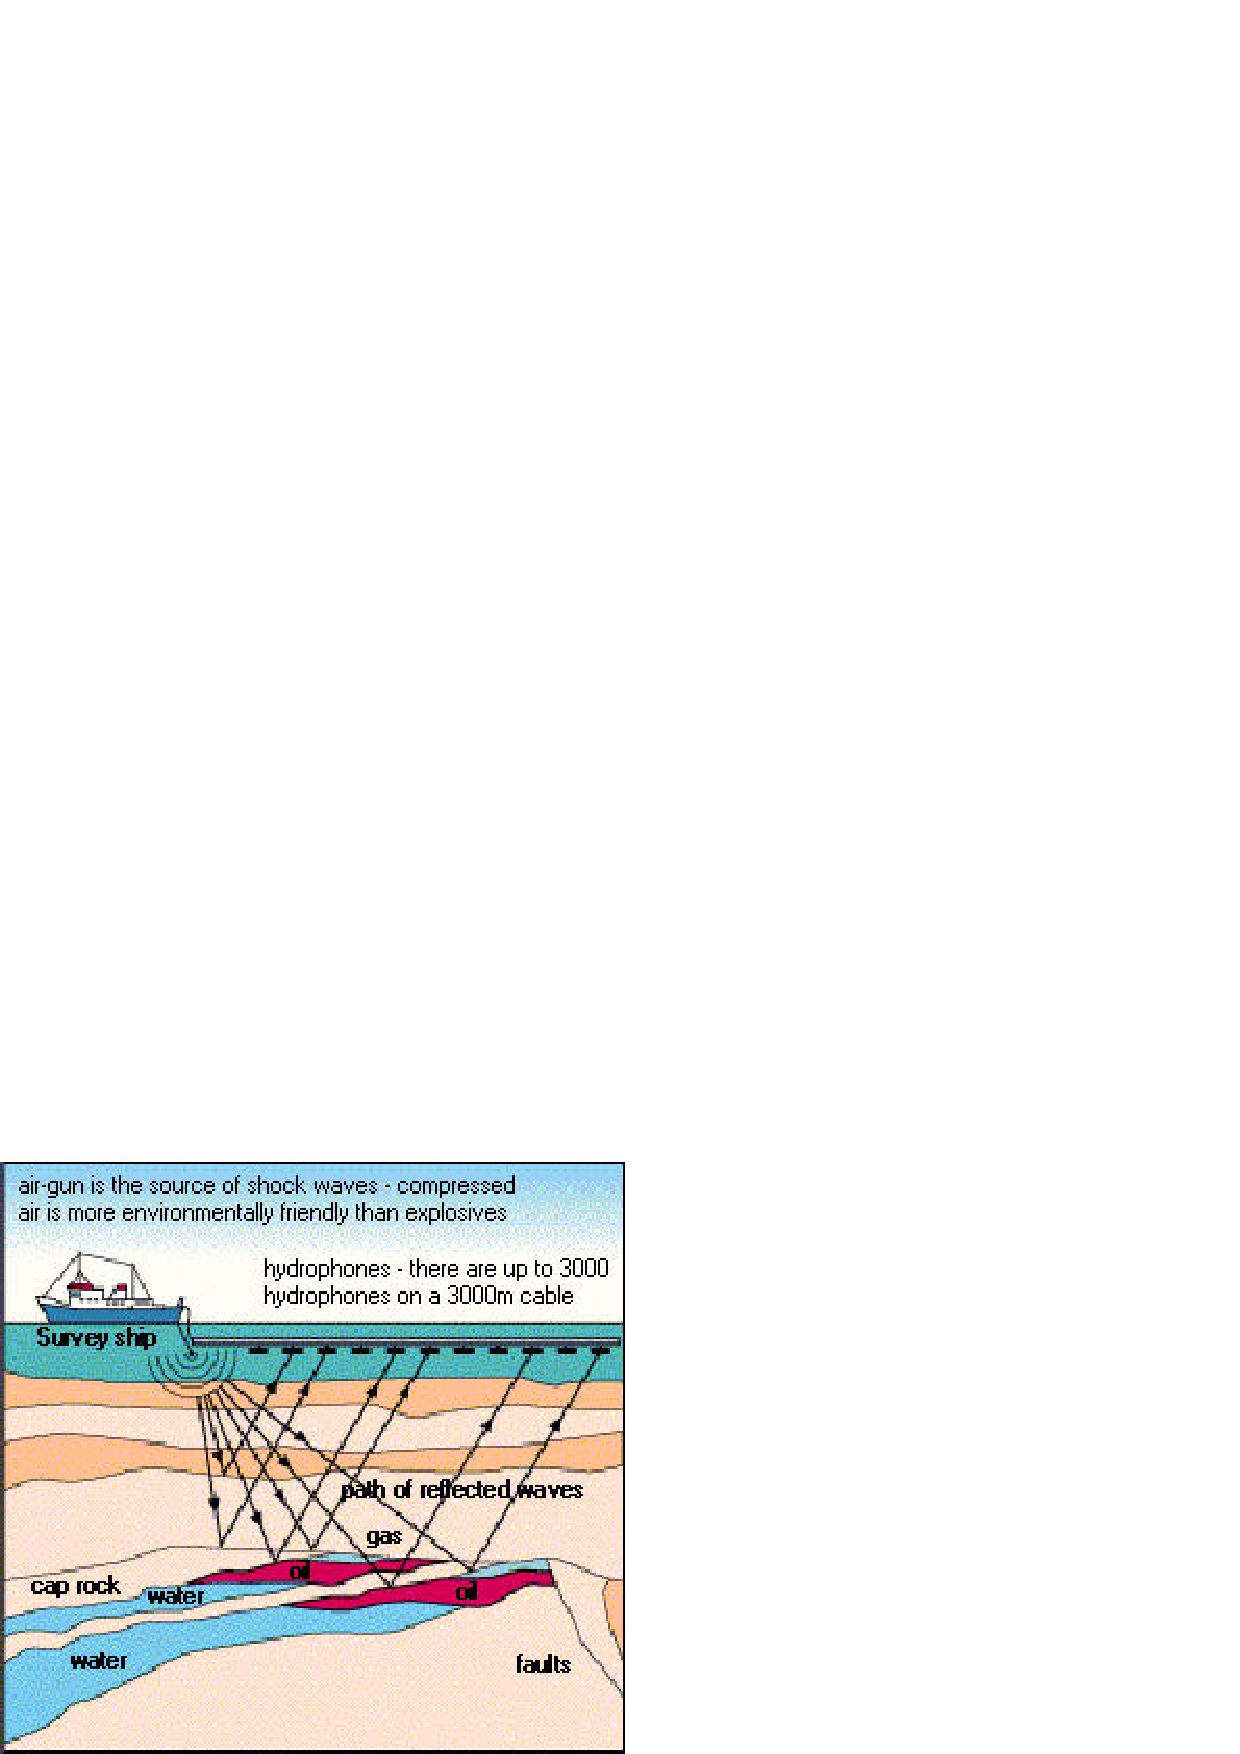
\includegraphics[scale=0.65]{img/oil-drilling-prospecting2.jpg}
\caption{Searching for oil over water using seismology}
\label{fig:oil-drilling}
\end{figure}

Here,
the survey ship excites seismic waves by its air gun, and the resulting
primary reflections are recorded by a set of hydrophones. The geologists
are the ones responsible for finding the oil trap or gas trap by processing
and analyzing the 3D wave fields that are reflected back by the subsurface.
However, only with the help of computers and engineers could the data
be processed and analyzed because terabytes of data would be processed.
The computational performance plays an important role through out
the process because the Reverse Time Migration (RTM) algorithm is
a high computational-demanding imaging algorithm.%
\footnote{The complexity of RTM for a single shot is roughly \BigO{n4}%
}



The ultimate and perhaps unattainable goal of computer science is
to make the computer to do whatever we want in perfect accuracy, speed,
security and on and on. Over time, the number of transistor on integrated
circuit doubles approximately every two year, which greatly improves
the computational performance and memory capacity of the general purpose
computer. However, as CPU speeds and memory capabilities have increased,
other aspects of performance, such as the access speed of register
and memory, or the access speed of memory and disk, have failed to
keep up. As a result, the performance of the whole system isn't likely
to improve a lot, and the access latencies frequently become a bottleneck
in the system.

Lots of efforts have been made facing with the access latencies, and
some of the methods gained extraordinary achievement. For example,
the vendors who manufacturing the chips try to use \emph {out-of-order
execution}  paradigm to make use of instruction cycles that would
be otherwise be wasted by a certain type of costly delay. One more
well-known ways to reduce the latencies between the fast-speed CPU
registers and relative-low-speed main memory is use \emph {caching.}
By storing the copy of data that are frequently accessed by the
processor into the cache, the amount of time that processors read
and write directly from/to memory decrease significantly, thus improves
the overall performance.

Such kinds of techniques, out-of-order execution, on-chip cache and
prefetching that we didn't mention before, does reduce the memory
latencies bottleneck, however, it also requires more transistors for
designing the processors, and the design of processors becomes more
and more complicated. What's worse, when the consecutive read/write
instructions cover a wide range of memory location, or the memory
access pattern is too random to predict, the application will suffer
from a high ratio of cache misses and the memory bottleneck re-emerge\cite{fu11}.

The current trend of improving the computer performance can be divided
into three category, increase the clock rate, fitting more and more
cores into a single processor, multiple computers (nodes) cooperate
together, and use some co-processors.

For years, processor makers consistently delivered increases in clock
rates and instruction-level parallelism, so that single-threaded code
executed faster on newer processors with no modification\cite{herb11}.
However, For a given device, operating at a higher clock rate always
requires more power. Especially, the high clock rate cannot be tolerated
in cluster computing or grid computing, or super computing, because
there are hundreds of thousands of processors within a cluster. That
is why the clock rate of servers servers generally stays between 2.0Ghz
and 2.4Ghz.

Now, to manage the CPU power dissipation, processor makers favor multi-core
designs, that is, integrate more than one core into a single processor,
such as the Intel Ferry CPUs, which have up to 32 cores. Following
the change of the CPU architecture, the software has also to be changed
at the same time. The previously single-thread (single-process) programs
have to be modified to multi-thread (multi-process) manner to take
full advantage of the hardware. Most of the multi-threaded development
paradigms introduce new overhead, and you will not see a linear increase
in speed vs number of processors. This is particularly true while
accessing shared or dependent resources, due to lock contention. This
effect becomes more noticeable as the number of processors increases\cite{moore}.

The computational performance for a single computer (node) is not
enough to support most of the science computation. Generally, scientists
and some of the industries would set up a \emph{cluster}, which consists
of a set of loosely connected or tightly connected computers that
work together so that in many respects they can be viewed as a single
system. Compared with a personal computer, the whole cluster certainly
has higher performance, but it also costs more power and the average
performance of a single node of the cluster is much lower than that
works individually. The entire performance of the cluster may even
increase slower when the number of nodes increase. What's more, for
a cluster, more aspects should be taken into consideration for tunning
the performance, including networking bandwidth and latency, parallel
file system performance, the application scalability and so on.

The most powerful supercomputer \emph{Titan}, which is made by Cray
Inc, has 560640 cores, 710144GB memory and it reaches high a Linpack
Performance of 17590.0 TFlops\footnote {Flops: number of double-precision
floating point operation per second} with its power being 8209kw\cite{top500}.
The scientist yet seems not content with the current computational
power because even by using the super computer, it still takes several
months or even several years to run some of simulation, such as seismic
imaging, weather simulation, ocean simulation, or global simulation.
And they need higher computational performance for a higher resolution
of the simulation.

Some vendors manufacture co-processor to aid CPU to better perform
general computing. For example, the NVIDIA Cooperation publish its
GPU accelerating card, which consists of hundreds of core in a single
card \footnote{There are 512 cores in NVIDIA Fermi GPUs}. GPU is better at general arithmetic
computation than general purpose CPU not only because it has more
cores than CPU, but also because its ratio of FLOPS  to power is much
higher than CPU. It can save lots of power in a cluster. The NVIDIA Inc
provides a set of
API, eg. CUDA C, for programmer to develop applications running on
NVIDIA card. The programs running on GPU cards are similar to the
programs running to CPU. In a word, they are both software.

Some vendors and researches still trying to increase the computational
performance as well as the ratio of FLOPS to power. You may wonder
whether we can build our application in hardware level instead of
software level, which could satisfy the vendors and researchers' willing.
That is why FPGA emerged.

A \emph {field-programmable gate array} (FPGA) is an integrated
circuit that is designed to be configured by the customer or a designer
after manufacturing, thereby \emph {field-programmable.}

The magic of FPGAs is that the connections among the logic gates (the
actual circuit you need) are made at power-up by reading the configuration
instructions written into a bit file. Changing the file changes the
function of the FPGA.

In this paper, I present my FPGA-based solution for the Reverse Time
Migration (RTM) algorithm ~\cite{yoon03}, which is the most computationally-demanding
imaging algorithms in oil and gas exploration.

The Reverse Time Migration (RTM) is a wave equation depth migration
method. It offers insights into geology that were previously impossible
to interpret or understand using seismic data.

Conventional migration methods, generally, use standard wave equation
techniques with mathematical approximations assuming that wave field
propagate in only one field. RTM is a two-way migration solution that
more accurately implements the wave equation and provides an alternative
approach to migration with fewer compromises. RTM works by running
the wave equation forward in time for the source and backwards in
time for the receiver ~\cite{shafiq}.

The RTM algorithm generally needs to deal with source and receiver
3D wave field arrays at thousands of different time steps, which brings
the requirement to manipulate terabytes of data in disk or in memory.
The kernel of the RTM algorithm, which applies a large 3D stencil
over a 3D data cube, needs to access a wide range of memory locations
while computing the result of one point. In many cases, the computation
incurs a large number of cache misses and reduces the performance
significantly. These highly demanding memory access characteristics
of RTM form a 'memory wall' that keeps us from achieving high throughput
in common computer clusters ~\cite{fu11}.

In this work, by utilizing the great computing performance of FPGA
and enormous internal memory bandwidth of the FPGA, I manage to implement
the computationally-demanding Reverse Time Migration algorithm in
FPGA.


\section{Field Programmable Gate Array}

\subsection{An Overview of FPGA}
Field Programmable Gate Array (FPGA) is a type of integrated circuit (IC)
containing a matrix of logic cells that can be programmed by a user to act
as an arbitrary integrated circuit.

The first field programmable gate array is manufactured by Xilinx
in 1985. However, compared with the widespread of computers, FPGA
was primarily made use of in telecommunications and networking in
the 1990s due to both the sophistication and the volume of the production.

Using the pre-built logic blocks and
programmable routing resources, you can configure these chips to implement
custom hardware functionality in high performance. For example, one can implement a
interrupt controller, a digital filter or even a processor on the basic of
FPGA.

In the past, FPGA technology could be used only by
engineers with a deep understanding of digital hardware design. Thus FPGA is
not as widely use as general purpose processor around the world. But in
the recent years, some companies encapsulated the underlining details of
FPGA and rised several suits of development tools kits to provide a higher
abstract interface for develops. The developers who designing the FPGA now
just need to task in the software and compile them down to a configuration
file or bitstream that contains information on how to components should be
wired together, which makes the task much easier and more and more
developers devotes their energies to FPGA.

\subsection{The Architecture of FPGA}

A typical layout of FPGA, Figure (\ref{fig:fpga_arch}) is an array of
interconnected programmable logic blocks or configurable logic blocks. It
provides the designer with programmable logic blocks that contain the pool
of combinatorial blocks and flip-flops to be used in the design. Logic is
often used in conjunction with memory. Clock conditioning has also become
commonplace, and support in the form of Delay Locked Loops (DLLs). Phase
Locked Loops (PLLs) is also provided inside the same silicon chip. Finally,
an FPGA chip does not lead a solitary life isolated from the rest of the
world. It needs to be easily interfaced to other chips or external signals.
In order to make this interfacing easier, FPGA vendors have invested a
great deal of effort in enhancing the flexibility of the input/output
blocks behind the chip pads. Each pad can serve as an input, an output, or
both. The list of electrical standards supported is extensive, and novel
techniques for maximizing bandwidth, such as clocking data in using both
edges of the clock, are widely supported~\cite{fpgaintro}.

\begin{figure}
  \centering
  \includegraphics[scale=0.25]{img/fpga_arch.png}
  \caption{Typical structure of modern FPGA}
  \label{fig:fpga_arch}
\end{figure}

Xilinx is the largest vendors of modern FPGA , their latest product, such
as Spartan-3 generation, general consist of five fundamental programmable
functional elements, configurable Logic Blocks (CLBs), Input/Output Blocks
(IOBs), BLOCK RAM, Multiplier Blocks, and Digital Clock Manager (DCM).

\begin{itemize}

  \item \emph{Configurable Logic Blocks (CLBs)} contain flexible Look-Up
    Tables (LUTs) that implement logic plus storage elements used as
    flip-flops or latches. CLBs perform a wide variety of logical functions
    as well as store data.

  \item \emph{Input/Output Blocks (IOBs)} control the flow of data between
    the I/O
    pins and the internal logic of the device. IOBs support bidirectional
    data flow plus 3-state operation. Supports a variety of signal
    standards, including several high-performance differential standards.
    Double Data-Rate (DDR) registers are included.

  \item \emph{Block RAM} provides data storage in the form of 18-Kbit
    dual-port
    blocks.

  \item \emph{Multiplier Blocks} accept two 18-bit binary numbers as inputs
    and
    calculate the product. The Spartan-3A DSP platform includes special DSP
    multiply-accumulate blocks.

  \item \emph{Digital Clock Manager (DCM)} Blocks provide self-calibrating,
    fully
    digital solutions for distributing, delaying, multiplying, dividing,
    and phase-shifting clock signals.
\end{itemize}

These elements are organized as shown in Figure (\ref{fig:spartan_arch}),
using the Spartan-3A FPGA
array as an example. A dual ring of staggered IOBs surrounds a regular
array of CLBs in the Spartan-3 and Extended Spartan-3A family. The
Spartan-3E family has a single ring of inline IOBs. Each block RAM column
consists of several 18-Kbit RAM blocks. Each block RAM is associated with a
dedicated multiplier. The DCMs are positioned with two at the top and two
at the bottom of the device, plus additional DCMs on the sides for the
larger devices.

\begin{figure}[h]
  \centering
  \includegraphics[scale=0.3]{img/spartan_arch.png}
  \caption{Spartan-3A Platform Architecture}
  \label{fig:spartan_arch}
\end{figure}

The Spartan-3 generation features a rich network of traces that
interconnect all five functional elements, transmitting signals among them.
Each functional element has an associated switch matrix that permits
multiple connections to the routing\cite{fpgaug}.

\subsection{Designing FPGA with Maxcompiler}

The usual way to design FPGAs is to write a behavioral model in
a Hardware Description Language (HDL), like Verilog or VHDL, which
supports concurrency and synchronous circuits. Concurrency allows
you to create fully parallel, independent processes, each describing
how to update some variables continuously. Synchronous circuits, instead,
are those made of flip-flops that change their state only on the edge
of some clock signal.

After the design has been written and verified with an HDL simulator,
a compiler creates a list of all the logic gates and the wires (nets)
that must connect them to reproduce the functionality of the HDL model.
After this logic synthesis, layout programs read the netlist and several
constraints files to find out which logic gates inside the FPGAs must
be used and which physical, internal wires must connect them to each
other. The end result is the bit file that the FPGA reads at power-up.

The above kind of FPGA configuring developing is still an obstruct for
those who seldom care much about hardware or digital circuit. In order to
make full use of FPGA, Maxeler Inc, develops a compiler where software
engineer can perform configuring developing with their daily used
developing language, such as C, and Java.

\subsubsection{Maxeler Acceleration Technology}

\emph{Maxcompiler} is a commercial product that is manufactured by Maxeler.
It is a compiler system for Maxeler hardware acceleration solutions using
FPGAs. The compiler system is a good assistant for software engineering
developer to create FPGA configuring because it has a higher abstract of
the underlining subtle hardware information, and then provide a set of
Application Interface for developers.

Figure (\ref{fig:maxeler_acceleration_system}) have a sketch of Maxeler
acceleration system architecture. The system comprises several FPGAs
attached directly to the local memory and to a host CPU via PCI Express.

\begin{figure}
  \centering
  \includegraphics[scale=0.35]{img/overview_of_maxeler_acceleration_system.png}
  \caption{An overview of Maxeler acceleration system}
  \label{fig:maxeler_acceleration_system}
\end{figure}

While developing the application, develops identify the runtime intensive part
and tunning them into FPGA configuration, which is called \emph{kernel} and
\emph{manager} in the acceleration system. After all the configured FPGA
files are compiled and downloaded into FPGA EEPROM, the host (CPU) code
communicate with FPGA with the help of \emph{Maxeler OS}. The Maxeler OS
provide a set of API called \emph{MaxCompierRT}, a runtime library to load
the configuration to FPGA and transfer data from/to FPGA.

The programming paradigm of FPGA designing is different from the general
programming paradigm, such as C/C++. The FPGA gains it high efficiency from
the parallel working of the different Configurable Logic Block (CLB). The
program describes the computations structurally (in space) rather than
specifying the sequence of processor instructions (in
time)\cite{max_white_paper}.

\subsubsection{Development Flow}
If the developer want to accelerate an application after he identifies the
runtime intensive part of the program, what he needs includes three parts,
designing the kernel, manager configuration and adapt the host application.
All the three parts can be easily implemented with the help of Maxeler
compiler tools. Figure (\ref{fig:development_flow}) presents the development flow with the main
components of MaxCompiler.

\begin{figure}[h]
  \centering
  \includegraphics[scale=0.4]{img/development_flow.png}
  \caption{Maxeler development flow}
  \label{fig:development_flow}
\end{figure}

The first stage, designing the kernel, is the most critical part of the
acceleration. Kernel has the similar meaning with that in CUDA GPU
programming, which refers to the most computationally-demanding part that
should be executed in the FPGA/GPU board. Java, the well-known high level
language is used to develop the kernel. Here we just the syntax of Java,
excluding the massive Java library. In addition, the Maxeler provides a set
of library that use to configure the kernel with the help of the
MaxCompiler. Instead of using the phase ``programming to configure kernel
with Java'', it is more appropriate to say ``designing the configure kernel
with Java'', because paradigm of designing the FPGA application with
MaxCompiler is to describe the structure of the logic, rather than telling
the FPGA the sequence of the process instructions, which we use in the
general purpose programming.

When the kernel is well configured, we need to set up a manager for it. The
manager is responsible for how to set up the kernel, for example, pass the
parameter to kernel that kernel expects. What's more, the manager is also
responsible to cooperate the kernels together if there are multiple
kernels, or multiple FPGA boards working for the same problem. The manager
can configure the kernel for simulation or for real work kernel.
Configuring the kernel for simulation is preferred because it saves time to
generate it. A full hardware build may take you hours or even weeks
depending on the complexity of the kernel.

Whenever the simulation kernel or the hardware kernel is build, it is
possible to linked it with the host application. Maxeler provides a set of
runtime library in C/C++ and Fortran to help the programmer to develop. The
communication between the local machine and FPGA device is via the runtime
library and interface, which could help the developer to transform data
from/to the FPGA Device.

The MaxCompiler can link them together in the last stage of the compilation
and generate the ordinary binary executable file.

\subsection{Advantage of FPGA Designing}

FPGA chip adoption across all industries is driven by the fact that FPGAs
combine the best parts of ASICs and processor-based systems. FPGAs provide
hardware-timed speed and reliability, but they do not require high volumes
to justify the large upfront expense of custom ASIC design. Reprogrammable
silicon also has the same flexibility of software running on a
processor-based system, but it is not limited by the number of processing
cores available.

Unlike processors, FPGAs are truly parallel in nature, so
different processing operations do not have to compete for the same
resources. Each independent processing task is assigned to a dedicated
section of the chip, and can function autonomously without any influence
from other logic blocks. As a result, the performance of one part of the
application is not affected when you add more processing.

In addition, FPGAs are blurring the lines between hardware and software in systems.
FPGA devices are inherently soft-programmable and may be changed
dynamically during the operation of a system. More compellingly, FPGA devices
now also contain embedded microprocessors within the logic fabric,
and these microprocessors can run Linux. Imagine a Linux computer
with up to millions of gates of flexible logic immediately around
it. One way to grok this new paradigm is to think of the following:
Software is configuration bits for hardware.


\section{Seismic Migration}

The purpose of the \emph{seismic exploration} is to understand the
constitution of the interior earth as much as possible. As we know, it is
impractical or even impossible to penetrate the earth and put your camera
there to capture the image, other indirect approaches are used to attain
the similar or same result. These approaches includes seismological
measurement, electromagnetic measurement and gravity measurement. As these
approaches are indirect, they usually give a analyze or indication of the
measured result. Some tools, such as computers, are required as part of the
analyze and the capability of the tools may be the bottleneck of the
analyze. For example, in the past, with the poor computational performance
of the computer, the data in only a small region and in a low resolution
could the seismologists analyzed due to the limited computing power.

As the Moore's Law indicates that the number of transistors double every 18
months, the computer gains much more computing power than before. Some
seismological method, which are computationally-demanding, seems not
practical in the past, can be implemented by utilizing the advanced
technology today. One of the most useful but computationally-demanding
algorithm, Reverse Time Migration algorithm, also comes into reality.

Reverse Time Migration is an algorithm of seismic migration. And seismic
migration is one of the most important part of seismic exploration, and
more specifically, seismic imaging. By seismic migration, the constitution
of the interior earth could be imaged, sketching, for example, the water,
rocks, gas, oil, faults etc in the subsurface.

\subsection{General Process of Seismic Exploration}

Seismic exploration, as one of the background knowledge of this thesis,
is explained in this section. Figure \ref{fig:sea_floor_seismic} shows a
typical scenario of a marine
based seismic exploration. The vessel will inject waves periodically by the
air gun. The waves just injected will spread in all direction quickly until
it penetrate different media, such as rocks, ands, gas, or oil beneath the
water, where the waves will reflect back or refract through another medium.
The reflected waves, or those refracts first, then reflected waves would be
recorded by an large array of Geo phones. In figure
\ref{fig:sea_floor_seismic}, another smaller ship shows up, dragging a
cable
which contains an array of sensors to record the reflected signals.

\begin{figure}
  \centering
  \includegraphics[scale=0.5]{img/Seafloor_Seismic.png}
  \caption{Marine-based Seismic Exploration}
  \label{fig:sea_floor_seismic}
\end{figure}

Geophysics data processing then follows the process of recording the
signals. First of all, multiple steps should be applied to perform the
preprocessing. For example, use the bandpass filter to remove the noise.
And last of all, is the migration step to reconstruct the image of
subsurface.

The detail of how the data are processed is not the topic of this thesis,
so I won't explain it too much. Those who are interested in the subject can
find more information with the help of the search engine. In this thesis, I
only concern about what is relevant with the FPGA implementation of the
computational part, which is explained in next subsection.

\subsection{Reverse Time Migration}

In this subsection, I present a general introduction for Reverse Time
Migration with some seismic terminologies. Revere Time Migration use the
source and recorded signals as input, following a series of computing, then
produce an image of the velocity model, which can maps to the real image of
the interior earth.

You may wonder why the velocity can be mapped to the real constitution of
the interior earth. There are several different objects inside the earth,
such as water, rocks, salt, gas, oil and they are the medium while the wave
propagating through them. The speed of the wave, usually the acoustic wave,
varies from the different medium, for example, the speed of sound is nearly
340 meter per second at temperature 20 degree. If we can generate a model
of the speed inside the earth, we can infer what is inside the earth.

The conventional one-way pre-stack depth migration approach, works well in
the layer medium, shown in Figure \ref{fig:layer_structure}. If the desired
layer, such as the gas or the oil lies horizontally, it can be easily
discovered with the conventional approach.

\begin{figure}[h]
  \centering
  \includegraphics[scale=.45]{img/layer_structure.jpg}
  \caption{Layered structure of the interior earth}
  \label{fig:layer_structure}
\end{figure}

However, not all desired resources are exposed in such a friendly form.
There may be some hill or large rocks beneath the sea, which will obstruct
the desired resource. In addition, some resources will stay in vertical
form or other forms instead of the restrict horizontal form. The
conventional one-way pre-stack depth migration approach could not handle
the previous situation. Thus why Reverse Time Migration emerged.

Reverse Time Migration algorithm is not a new algorithm, instead, it is
first put forward in the 1970s. However, people at that time thinks that it
is impractical or impossible to use such algorithm in practice due to the
tensive  computation requirement. But nowadays, it is impossible to
implement the Reverse Time Migration thanks to the fast developing of
computers.

Instead of just one-way pre-stack depth migration, the Reverse Time
Migration is a two-way pre-stack depth migration, which handles steeply
dipping events, turning waves and multiples. The detail of the algorithm
will be explained in the next section.

Figure \ref{fig:comparison} show an introductory example with synthetic
data that illustrates the potential power of the Reverse Time Migration.
There are mainly two part of object in the model, one is water (color from
blue to yellow), the other one is salt (color in red). The figure in the
left is not a real image of the interior earth, but a velocity of that
zone. As the water gets deeper, the speed of the sound becomes faster, so
that is why the color turns from blue to yellow and dark yellow. The salt
is solid object, where the speed of sound is much faster than that in the
water, so the color is in red, a darker color than yellow.

\begin{figure}[h]
  \hfill
  \includegraphics[scale=.25]{img/velocity_model.png}
  \caption{Synthetic comparison of salt flank}
  \label{fig:comparison}
\end{figure}

Concerning about the result, we take a comparison of the middle and right
one in Figure \ref{fig:comparison}. The middle one is generated using the
one-way wave equation. It is obvious that the salt flank below the overhang
is poorly imaged. On real data, it is difficult to understand the dip and
the structure of sedimentary strata in similar overhang zone. Thus the
potential existence of gas or oil against the salt are impossible to
identify. On the other hand, the last figure, which is produced using the
RTM algorithm, yielding a big improvement. It has a clear profile that is
similar to the original synthetic data.

\section{RTM Algorithm and Analysis}

As it is mentioned in the previous section that the Reverse Time Migration
algorithm can gain a big improvement but it is computationally demanding.
In this section, we have a look at the detail of the algorithm and present
a computation complexity analyze of it.

The main steps of the algorithm is explained as below\cite{rtm}.

\begin{enumerate}
\item the forward extrapolation of a modelled source waved for each shot
  location through a gridded velocity model is performed. And the wave
  field at each time step is saved for later application of the ``imaging
  condition''.
\item the receiver wave field for each shot, which is recorded in the
  field, is backward propagated in time through the same velocity model.
\item at each time step, the corresponding source and receiver wave fields
  are correlated by applying the imaging condition. Thus, the final
  wave field in the source propagating scheme is correlated with the
  initial wave field in the receiver propagation scheme, and so on backward
  through the receiver propagation.
\item the result are summed to form a partial image volume for each shot.
\item the image volumes for consecutive gathers are spatially summed to
  produce the final pre-stack depth image.
\end{enumerate}

So, now you may know why RTM is so computation expensive and has several
decades to be commercially implemented.

\subsection{Mathematical Derivation of RTM}

If we assume that the wave that the wave injects is acoustic wave (sound
wave), then we can use the acoustic wave equation as the first step of the
derivation.

\begin{equation}
  \frac{1}{c^2}\cdot\frac{\partial ^2u}{\partial t^2}=\bigtriangledown ^2u +s
\end{equation}



%% The following contains your structure of your thesis and your
%% contribution, comparison with CPU version.


% include the bibliography
\begin{thebibliography}{9}
    \bibitem{fu11} H. Fu and R. G. Clapp, \emph{Eliminating the memory
    bottleneck: an FPGA-based solution for 3d reverse time migration,}
    in Proceedings of the 19th ACM/SIGDA international symposium on Field
    programmable gate arrays, 2011, pp. 65-74.

    \bibitem{herb11} Herb Sutter, \emph{The Free Lunch Is Over: A Fundamental
    Turn Toward Concurrency in Software,} Dr. Dobb's Journal, 30(3), March
    2005. Retrieved 21 November 2011.

    \bibitem{yoon03} K. Yoon, C.Chin, S. Suh, L. Lines, and S. Hong.
    \emph{3D Reverse-time Migration Using the Acoustic Wave Equation:
    An Experience with the SEG/EAGE Data Set.} The Leading Edge, 22(1):38-41,
    2003.

    \bibitem{moore} Moores law, Wikipedia, the free encyclopedia.

    \bibitem{shafiq} M. Shafiq, M. Pericas, N. Navarro, and E. Ayguade,
    \emph{A Streaming Based High Performance FPGA Core for 3D Reverse
    Time Migration.}

    \bibitem{top500} Top500 List - November 2012

    \bibitem{fpgaintro}
    J. Serrano,
    \emph{DIGITAL SIGNAL PROCESSING USING FIELD PROGRAMMABLE GATE ARRAYS,}
    Proceedings of BIW08, pp. 29-38, 2008.

    \bibitem{fpgaug}
    Xilinx Inc,
    \emph{FPGA USER GUIDE}

    \bibitem{max_white_paper}
    MaxCompiler White Paper

    \bibitem{rtm}
    Reverse Time Migration

\end{thebibliography}

%\begin{thebibliography}{9}
    \bibitem{fu11} H. Fu and R. G. Clapp, \emph{Eliminating the memory
    bottleneck: an FPGA-based solution for 3d reverse time migration,}
    in Proceedings of the 19th ACM/SIGDA international symposium on Field
    programmable gate arrays, 2011, pp. 65-74.

    \bibitem{herb11} Herb Sutter, \emph{The Free Lunch Is Over: A Fundamental
    Turn Toward Concurrency in Software,} Dr. Dobb's Journal, 30(3), March
    2005. Retrieved 21 November 2011.

    \bibitem{yoon03} K. Yoon, C.Chin, S. Suh, L. Lines, and S. Hong.
    \emph{3D Reverse-time Migration Using the Acoustic Wave Equation:
    An Experience with the SEG/EAGE Data Set.} The Leading Edge, 22(1):38-41,
    2003.

    \bibitem{moore} Moores law, Wikipedia, the free encyclopedia.

    \bibitem{shafiq} M. Shafiq, M. Pericas, N. Navarro, and E. Ayguade,
    \emph{A Streaming Based High Performance FPGA Core for 3D Reverse
    Time Migration.}

    \bibitem{top500} Top500 List - November 2012

    \bibitem{fpgaintro}
    J. Serrano,
    \emph{DIGITAL SIGNAL PROCESSING USING FIELD PROGRAMMABLE GATE ARRAYS,}
    Proceedings of BIW08, pp. 29-38, 2008.

    \bibitem{fpgaug}
    Xilinx Inc,
    \emph{FPGA USER GUIDE}

    \bibitem{max_white_paper}
    MaxCompiler White Paper

    \bibitem{rtm}
    Reverse Time Migration

\end{thebibliography}


\end{document}
